From a user's point of view, \Mimir\ is a tool for searching a collection of
semantically annotated documents.  It provides facilities for searching over
different views of the document text, for example one can search the document
words, the part-of-speech of those words, or their morphological roots. Beside
searching the document text, \Mimir\ also supports searches over the documents'
semantic annotations, where queries are based on annotation types and
restrictions over the values of annotation features. These different search
paradigms can be combined freely into complex queries, with support for
sequences, repetitions, and Boolean operators.

A search session entails the formulation of a query, running the query with the
\Mimir\ query engine, and consuming the query results.  \Mimir\ queries are
expressed in a text-based query language which is described in
section~\ref{sec:search:ql}.  The way these queries are submitted to \Mimir\
depends on how it is deployed, the various interfaces are discussed in
section~\ref{sec:search:interfaces}.


\section{The \Mimir\ query language}\label{sec:search:ql}

A \Mimir\ query is either a simple query (i.e. a {\tt String} query,
section~\ref{sec:string-query}, or an {\tt Annotation} query,
section~\ref{sec:annotation-query}), or a compound one, which comprises a set of
sub-queries linked by operators. If no operator is placed between any two
sub-queries, then the {\tt Sequence} operator (see
section~\ref{sec:sequence-query}) is implied. This means that several queries
written one after another are interpreted as one sequence query. For example, a
query like `{\it the brown dog}' is interpreted as a sequence query, having
three sub-queries, each of them being a String query. This would match
occurrences of the exact phrase `{\it the brown dog}' in the indexed documents.
Note that this is different from the standard behaviour of search engines,
which would simply match documents in which all three query terms occur, in
whichever order. That type of search is also supported in \Mimir, through the
{\tt AND} operator (see section~\ref{sec:and-query}).  Parentheses can be used
for grouping where the syntax would otherwise be ambiguous.

\subsection{String Queries}\label{sec:string-query}

The simplest form of query is a query term. This will match all occurrences of
the query term in the indexed documents.

If the \Mimir\ index being interrogated includes multiple token indexes, then
the particular index to be searched can be specified by prefixing the query
term with the index name and a colon, for example the query
`{\it root:be}'\footnote{This assumes that an index named {\tt root} exists,
and was used to store the morphological root of the words.} will match all
morphological forms of the verb {\it to be}. If the name of the string index is
omitted, then the first configured index is used. By convention (reflected in
the default \Mimir\ configuration) the first string index is used to store the
terms text, so the default behaviour is to search over the document text, as
expected.  Double-quoted strings are treated as plain term queries against the
first token index in a similar way.

In fact the above is a slight simplification, as bare terms (and double-quoted
strings) are actually tokenised before being searched for.  This is because
\Mimir\ views documents as streams of tokens, not characters, and the query
must match the tokenisation that was used to index the documents.  For example,
the default GATE tokeniser treats ``don't'' as two tokens, ``do'' and ``n't'',
so a query for {\em don't} as a single token would fail.  To get around this,
\Mimir\ runs a GATE application over the string of the query to generate
Token annotations, and then constructs a query for these tokens in sequence
(see section~\ref{sec:sequence-query}).  Named index queries (``root:be'') are
not tokenised, so if you want to avoid tokenising a particular query for any
reason (e.g. if you suspect there is a mis-tokenised document in your index)
you can explicitly name the appropriate index (typically ``string'', i.e.
string:don't).

\subsubsection{Annotation Queries}\label{sec:annotation-query}

If annotation indexes were used during indexing, \Mimir\ allows searching for
annotation-based patterns. An annotation is a piece of metadata
associated with a text segment, with a {\bf type} and optionally
{\bf features}.  An annotation query takes the following form: 
{\tt \{Type feature1=value1 feature2=value2 \ldots\}}.  The annotation type is
required, the feature constraints are optional.

While the example above uses equality for the feature constraints, other
operators are also available. Here is the full list:
\bde
  \item[equality:] represented by the sign $=$, matches annotations which have
  the given value for the specified feature. The equality operator is
  applicable to features of any type.
  \item[comparison operators:] represented by one of the following symbols:
  $<$, $<=$, $>$, $>=$, with the usual meaning. These operators can apply to
  features of type {\tt nominal}, {\tt numeric}, or {\tt text}.
  \item[regular expressions:] can be specified using the syntax {\tt
  REGEX(pattern, flags)}, where the {\tt pattern} represents the regular
  expression sought, and the {\tt flags} are optional, and can be used to
  change the way matching is performed. See
  \url{http://www.w3.org/TR/xpath-functions/#regex-syntax} for a full
  specification of the regular expression support. The {\tt REGEX} operator can
  only be used for {\tt nominal}, and {\tt text} features.
\ede

Examples:\\
\{Person gender $=$ female\} -- searches for annotations of type
{\tt Person}, which have a feature named {\tt gender}, with the value
{\it female}.

\{Measurement type $=$ scalar normalisedValue $>0$ normalisedValue $<10$
normalisedUnit $=$ m\} -- searches for scalar measurements, with a unit of {\it
metre}, and a normalised value between $0$ and $10$\footnote{The extended
support for Measurement annotations is discussed further in
section~\ref{sec:plugins:measurements}.}.  Note that the same feature name
can be used in several constraints, in which case only annotations where the
feature meets {\em all} the constraints will be matched by the query.  For
disjunctive queries, use the OR operator described below.

In order to be able to search on a particular feature, that feature
must have been specified in the index template when the index was created --
\Mimir\ indexes only the features it has been told to index.  There may be
additional ``synthetic'' features available at query time depending on the
semantic annotation helper that the index uses for the given annotation type,
for example the SPARQL helper allows queries on the ``feature'' named
``sparql'', the measurements helper allows queries for ``spec'' etc.

\subsection{AND Operator: ``{\tt \&}''}\label{sec:and-query}

The `{\tt AND}' (also `\&`) operator can be used to specify queries that should
match document segments that include at least one hit from each of the
sub-queries. The results returned will always be the shortest document segments
that satisfy the query.

\subsection{OR Operator: ``{\tt |}''}\label{sec:or-query}

{\tt OR} queries are used to search hits that match one of a set of alternative
query expressions. This is indicated by using the {\tt `OR'} (also`\verb!|!')
operator between the sub-queries. A query of the form {\tt Query1 | Query2} will
return hits that match either sub-query {\tt Query1} or sub-query {\tt Query2}.

\subsection{IN and OVER Operators}\label{sec:containment-query}

The operators {\tt IN} and {\tt OVER} are used to search for hits of a query
that contain, or are contained in the hits of another query. For example:
\begin{description}
\item[Query1 IN Query2] will match all the hits of {\tt Query1} that are
contained in a hit of {\tt Query2}.
\item[Query1 OVER Query2] will match all hits of {\tt Query1} that contain (are
overlapping) a hit of {\tt Query2}.
\end{description}

\subsection{Repeats Operator: ``+''}\label{sec:kleene-query}

The $+$ operator can be used to match text segments that comprise a sequence of
hits from the same sub-query. The length of the sequence is specified though a
number (representing the {\bf maximum} number of repetitions) or through two
numeric values (representing the {\bf minimum} and {\bf maximum} number of
repetitions). For example:
\bde
  \item[{\tt to+3}] will match one, two, or three repeated occurrences of the
  word {\it to}. The returned hits will be of the form ``{\it to}'', ``{\it to  
  to}'', or ``{\it to to to}'').
  \item[{\tt \{Person\}+2..5}] will match sequences of 2, 3, 4, or 5
  adjacent {\tt Person} annotations.
  \item[{\tt (\{Location locType = city\} |
  \{Location locType = country\})+3}] will match any sequence of up to
  three Location annotations where each one refers to either a city or a
  country.
\ede

Note that there is no support for a repetition count of zero (an optional
match) -- you will need to reformulate the query to cover the versions with and
without the optional match separately and combine them with an OR, for example
{\tt (term1 term2+2 term3) | (term1 term3)}.  Similarly there is no support for
unbounded wildcards ({\em n} times or more).

\subsection{Sequence Queries and Gaps}\label{sec:sequence-query}

As sequence is the default operator in \Mimir, there is no graphical sign for
it: simply writing a set of queries one after another will cause a search for
sequences of hits, one from each sub-query. For example, the query ``{\tt the
energy level}'' is actually a sequence query where the first sub-query searches
for the word ``{\it the}'', the second for ``{\it energy}'', and the last for
``{\it level}''.

It is sometimes useful to include gaps in a sequence query, that is to allow
arbitrary text fragments (of specified length) to occur in-between the hits
from some of the sub-queries. This can be done by using the gap markers ``{\tt
[n]}'', or ``{\tt [m..n]}''. These will match a sequence of length $n$, or with
a length of between $m$ and $n$ of arbitrary tokens.

For example the query ``{\tt the [2] root:time}'' will match phrases like ``{\it
the best of times}'' or ``{\it the worst of times}'', whereas the query ``{\tt
the [2..10] root:time}'' would also match ``{\it the best use of one's time}''
(where the gap consists of six tokens -- five words and an apostrophe).

\subsection{Escaping Reserved Words}

Some words are part of the query language definition so they cannot be used
directly as query terms. If that is desired, then these constructs must be
escaped as shown in the following table:
\begin{center}
\begin{tabular}{|l|l|}
\hline
{\bf Reserved input} & {\bf Escaped form}\\
\hline \hline
\{, \} &  $\backslash$\{, $\backslash$\}\\
\hline
(, )  & $\backslash$(, $\backslash$) \\
\hline
[, ] & $\backslash$[, $\backslash$]\\
\hline
: &  $\backslash$: \\
\hline
+ &  $\backslash$+ \\
\hline
{\tt |} &  $\backslash${\tt |} \\
\hline
{\tt \&} &  $\backslash${\tt \&} \\
\hline
? &  $\backslash$? \\
\hline
$\backslash$ &  $\backslash$$\backslash$ \\
\hline
. &  $\backslash$. \\
\hline
" &  $\backslash$" \\
\hline 
=  & $\backslash$= \\
\hline
IN & ``IN'' \\
\hline
OVER & ``OVER''\\ 
\hline
OR & ``OR''\\ 
\hline
AND & ``AND''\\ 
\hline
\end{tabular}\\
\vspace{1ex}
Escaping reserved constructs in the \Mimir\ query language
\end{center}

%%%%%%%%%%%%%%%%%%%%%%%%%%%%%%%%%%%%%%%%%%%%%%%%%%%%%%%%%%%%%%%%%%%%%%%%%%

\section{Search interfaces -- how to submit queries to \Mimir}
\label{sec:search:interfaces}

The \Mimir\ Grails plugin supplies two search interfaces by default, with the
infrastructure to implement other interfaces as required.  An XML-based service
interface allows other applications to submit queries to the indexes hosted by
a \Mimir\ web application by POSTing requests over HTTP (described in
section~\ref{sec:search:service}).  There is also an example user-facing search
interface called {\em GUS}, intended primarily for testing and demonstration
purposes (described in section~\ref{sec:search:gus}).  Both of these interfaces
interact with the underlying indexes through the {\tt SearchService} Grails
service provided by the plugin.  When embedding the \Mimir\ Grails plugin in
another Grails application this service is the primary means for application
code to interact with \Mimir, and is described in
section~\ref{sec:search:grails}.

\subsection{\Mimir\ Search Web Service}\label{sec:search:service}

The \Mimir\ web application exposes the search functionality as a web service
that can be accessed through a simple HTTP interface. All requests are performed
by calling an action with a set of parameters; the results of a call are encoded
in XML and returned as the response to the request.  All the example URLs in
this section assume the {\tt mimir-demo} application with its
default URL mappings, running on {\tt localhost} port 8080.

The \Mimir\ web service can be accessed at a URL like:\\
{\tt http://localhost:8080/mimir-demo/\{index ID\}/search/\{action\}},
where the {\tt action} value is the name of one of the supported actions,
described below. The actual URL (with the correct index ID included) can be
obtained from the {\em index information page} presented by  the \Mimir\ web
application.  Parameters may be supplied as query parameters with a {\tt GET}
request or in normal {\tt application/x-www-form-urlencoded} form in a
{\tt POST} request.  Alternatively, they may be supplied as XML (if the request
content type is {\tt text/xml} or {\tt application/xml}) of the form:
\begin{verbatim}
<request xmlns="http://gate.ac.uk/ns/mimir">
  <firstParam>value</firstParam>
  <secondParam>value</secondParam>
</request>
\end{verbatim}

The first request to the service will return a session cookie, which must be
passed back with all subsequent requests.

When accessing the service URL with no value provided for {\tt action}, a help
page will be returned presenting the documentation associated with the XML web
service.

% Switch to compact listings mode
\lstcompact\

The following actions are available:\\
\begin{longtable}{|p{1.8cm}|p{10.2cm}|}
\multicolumn{2}{l}{\tt \bf help}\\
\hline
Function & Obtain service documentation.\\
\hline
Parameters & none\\
\hline
Returns & A help message describing how to use the service.\\
\hline
\end{longtable}

\begin{longtable}{|p{1.8cm}|p{10.2cm}|}
\multicolumn{2}{l}{\tt \bf postQuery} \\
\hline
Function & Starts a new query.  The query will execute asynchronously in a
background thread, and will initially run until it has found a maximum of 1
million hits or has been running for 30 seconds, whichever comes first.  If the
query runner hits one of these limits before the search is complete it can be
restarted by calling the {\tt getMoreHits} action. \\
\hline
Parameters & \begin{minipage}[t]{10.2cm}
\begin{description}
\item[queryString:]the text of the query, using the \Mimir\ query language.
\end{description}
\end{minipage}\\
\hline
Returns & \begin{minipage}[t]{10.2cm}
An XML message with the ID of the new query,
or an error message if there were any problems while parsing the query.

Example request:\\
\lstinline[language=XML]!http://localhost:8080/mimir-demo/a4300d00-2dd1-4797-8eaa-e65b0c7d879b/search/postQuery?queryString=%22the%22!

Example response:
\begin{lstlisting}[language=XML]
<?xml version="1.0"?>
<message xmlns='http://gate.ac.uk/ns/mimir'>
  <state>SUCCESS</state>
  <data>
    <queryId>a28656e2-18f4-4b58-b9d3-9a9378eb14d0</queryId>
  </data>
</message>
\end{lstlisting}
\end{minipage}\\
\hline
\end{longtable}

\begin{longtable}{|p{1.8cm}|p{10.2cm}|}
\multicolumn{2}{l}{\tt \bf hitCount} \\
\hline
Function & Obtains the number of hits collected so far. If a query is not
complete, more hits may be available at later time. If a query has stopped being
active before completing, it can be restarted by calling {\tt getMoreHits}.\\
\hline
Parameters & \begin{minipage}[t]{10.2cm}
\begin{description}
\item[queryId:]the ID for the query, as returned by the {\tt postQuery} action.
\end{description}
\end{minipage}\\
\hline
Returns & \begin{minipage}[t]{10.2cm}
An XML message encapsulating a numeric value, or an error message if there were 
any problems.

Example request:\\
\lstinline[language=XML]!http://localhost:8080/mimir-demo/a4300d00-2dd1-4797-8eaa-e65b0c7d879b/search/hitCount?queryId=a28656e2-18f4-4b58-b9d3-9a9378eb14d0!

Example response:
\begin{lstlisting}[language=XML]
<?xml version="1.0"?>
<message xmlns='http://gate.ac.uk/ns/mimir'>
  <state>SUCCESS</state>
  <data>
    <value>6257</value>
  </data>
</message>
\end{lstlisting}

Example error response:
\begin{lstlisting}[language=XML]
<?xml version="1.0"?>
<message xmlns='http://gate.ac.uk/ns/mimir'>
  <state>ERROR</state>
  <error>Query ID a28656e2-18f4-4b58-b9d3-9a9378eb14d1 not known!</error>
</message>
\end{lstlisting}
\end{minipage}\\
\hline
\end{longtable}

\begin{longtable}{|p{1.8cm}|p{10.2cm}|}
\multicolumn{2}{l}{\tt \bf docCount} \\
\hline
Function & Obtains the number distinct documents that have been found so far
to contain hits.\\
\hline
Parameters & \begin{minipage}[t]{10.2cm}
\begin{description}
\item[queryId:]the ID for the query, as returned by the {\tt postQuery} action.
\end{description}
\end{minipage}\\
\hline
Returns & \begin{minipage}[t]{10.2cm}
An XML message encapsulating a numeric value, or an error message if there were 
any problems.

Example request:\\
\lstinline[language=XML]!http://localhost:8080/mimir-demo/a4300d00-2dd1-4797-8eaa-e65b0c7d879b/search/docCount?queryId=a28656e2-18f4-4b58-b9d3-9a9378eb14d0!

Example response:
\begin{lstlisting}[language=XML]
<?xml version="1.0"?>
<message xmlns='http://gate.ac.uk/ns/mimir'>
  <state>SUCCESS</state>
  <data>
    <value>11</value>
  </data>
</message>
\end{lstlisting}
\end{minipage}\\
\hline
\end{longtable}

\begin{longtable}{|p{1.8cm}|p{10.2cm}|}
\multicolumn{2}{l}{\tt \bf docStats} \\
\hline
Function & Obtains the statistics for the documents that have been found so far
to contain hits. These include the document IDs and the number of hits for
each individual document.\\
\hline
Parameters & \begin{minipage}[t]{10.2cm}
\begin{description}
\item[queryId:]the ID for the query, as returned by the {\tt postQuery} action.
\item[startIndex]the first requested document. A value of $0$ requests the
details for the first document found to contain hits.
\item[count]the number of documents for which the details are requested.  
\end{description}
\end{minipage}\\
\hline
Returns & \begin{minipage}[t]{10.2cm}
An XML message encapsulating a set of {\tt <document>} elements, one for
each individual document.

Example request:\\
\lstinline[language=XML]!http://localhost:8080/mimir-demo/a4300d00-2dd1-4797-8eaa-e65b0c7d879b/search/docStats?queryId=a28656e2-18f4-4b58-b9d3-9a9378eb14d0&startIndex=0&count=11!

Example response:
\begin{lstlisting}[language=XML]
<?xml version="1.0"?>
<message xmlns='http://gate.ac.uk/ns/mimir'>
  <state>SUCCESS</state>
  <data>
    <document id='0' hitCount='622'/>
    <document id='1' hitCount='300'/>
    <document id='2' hitCount='448'/>
    <document id='3' hitCount='273'/>
    <document id='4' hitCount='1053'/>
    <document id='5' hitCount='677'/>
    <document id='6' hitCount='86'/>
    <document id='7' hitCount='1399'/>
    <document id='8' hitCount='356'/>
    <document id='9' hitCount='841'/>
    <document id='10' hitCount='202'/>
  </data>
</message>
\end{lstlisting}
Note that as our query was simply {\it ``the''}, we have found hits on every
document. In a more typical case, not all document IDs will be represented in
the results.
\end{minipage}\\
\hline
\end{longtable}

\begin{longtable}{|p{1.8cm}|p{10.2cm}|}
\newpage\multicolumn{2}{l}{\tt \bf hits} \\
\hline 
Function & Obtains a set of hits. Each hit is defined by a document
ID, a position and a length, both of which are defined in terms of tokens, not
characters (see Section~\ref{sec:indexing:tokens} for details).\\
\hline
Parameters & \begin{minipage}[t]{10.2cm}
\begin{description}
\item[queryId:]the ID for the query, as returned by the {\tt postQuery} action.
\item[startIndex]the first requested hit. A value of $0$ requests the
details for the first hit found.
\item[count]the number of hits for which the details are requested.  
\end{description}
\end{minipage}\\
\hline
Returns & \begin{minipage}[t]{10.2cm}
An XML message encapsulating a set of {\tt <hit>} elements, one for
each individual hit.

Example request:\\
\lstinline[language=XML]!http://localhost:8080/mimir-demo/a4300d00-2dd1-4797-8eaa-e65b0c7d879b/search/hits?queryId=a28656e2-18f4-4b58-b9d3-9a9378eb14d0&startIndex=0&count=11!

Example response:
\begin{lstlisting}[language=XML]
<?xml version="1.0"?>
<message xmlns='http://gate.ac.uk/ns/mimir'>
  <state>SUCCESS</state>
  <data>
    <hits>
      <hit documentId='0' position='257' length='1'/>
      <hit documentId='0' position='266' length='1'/>
      <hit documentId='0' position='290' length='1'/>
      <hit documentId='0' position='303' length='1'/>
      <hit documentId='0' position='309' length='1'/>
      <hit documentId='0' position='316' length='1'/>
      <hit documentId='0' position='320' length='1'/>
      <hit documentId='0' position='332' length='1'/>
      <hit documentId='0' position='335' length='1'/>
      <hit documentId='0' position='342' length='1'/>
      <hit documentId='0' position='348' length='1'/>
    </hits>
  </data>
</message>
\end{lstlisting}
\end{minipage}\\
\hline
\end{longtable}

\begin{longtable}{|p{1.8cm}|p{10.2cm}|}
\multicolumn{2}{l}{\tt \bf getMoreHits} \\
\hline
Function & Requests a query that has stopped collecting hits before
completing to restart collecting hits. If the query has already completed, or
is already active, this call will simply be ignored (it will not cause an
error).\\
\hline
Parameters & \begin{minipage}[t]{10.2cm}
\begin{description}
\item[queryId:]the ID for the query, as returned by the {\tt postQuery} action.
\end{description}
\end{minipage}\\
\hline
Returns & \begin{minipage}[t]{10.2cm}
An XML message reporting success or failure.

Example request:\\
\lstinline[language=XML]!http://localhost:8080/mimir-demo/a4300d00-2dd1-4797-8eaa-e65b0c7d879b/search/getMoreHits?queryId=a28656e2-18f4-4b58-b9d3-9a9378eb14d0!

Example response:
\begin{lstlisting}[language=XML]
<?xml version="1.0"?>
<message xmlns='http://gate.ac.uk/ns/mimir'>
  <state>SUCCESS</state>
</message>
\end{lstlisting}
\end{minipage}\\
\hline
\end{longtable}

\begin{longtable}{|p{1.8cm}|p{10.2cm}|}
\multicolumn{2}{l}{\tt \bf isActive} \\
\hline
Function & Checks if a query is still working on collecting hits.\\
\hline
Parameters & \begin{minipage}[t]{10.2cm}
\begin{description}
\item[queryId:]the ID for the query, as returned by the {\tt postQuery} action.
\end{description}
\end{minipage}\\
\hline
Returns & \begin{minipage}[t]{10.2cm}
An XML message encapsulating a Boolean value, or an error message if there were 
any problems.

Example request:\\
\lstinline[language=XML]!http://localhost:8080/mimir-demo/a4300d00-2dd1-4797-8eaa-e65b0c7d879b/search/isActive?queryId=a28656e2-18f4-4b58-b9d3-9a9378eb14d0!

Example response:
\begin{lstlisting}[language=XML]
<?xml version="1.0"?>
<message xmlns='http://gate.ac.uk/ns/mimir'>
  <state>SUCCESS</state>
  <data>
    <value>false</value>
  </data>
</message>
\end{lstlisting}
\end{minipage}\\
\hline
\end{longtable}

\begin{longtable}{|p{1.8cm}|p{10.2cm}|}
\multicolumn{2}{l}{\tt \bf isComplete} \\
\hline
Function & Checks if a query has finished collecting all the hits. If a query
is not complete, more hits may be available at a later time. If a query has
stopped being active before completing, it can be restarted by calling {\tt
getMoreHits}.\\
\hline
Parameters & \begin{minipage}[t]{10.2cm}
\begin{description}
\item[queryId:]the ID for the query, as returned by the {\tt postQuery} action.
\end{description}
\end{minipage}\\
\hline
Returns & \begin{minipage}[t]{10.2cm}
An XML message encapsulating a Boolean value, or an error message if there were 
any problems.

Example request:\\
\lstinline[language=XML]!http://localhost:8080/mimir-demo/a4300d00-2dd1-4797-8eaa-e65b0c7d879b/search/isComplete?queryId=a28656e2-18f4-4b58-b9d3-9a9378eb14d0!

Example response:
\begin{lstlisting}[language=XML]
<?xml version="1.0"?>
<message xmlns='http://gate.ac.uk/ns/mimir'>
  <state>SUCCESS</state>
  <data>
    <value>true</value>
  </data>
</message>
\end{lstlisting}
\end{minipage}\\
\hline
\end{longtable}

\begin{longtable}{|p{1.8cm}|p{10.2cm}|}
\multicolumn{2}{l}{\tt \bf renderDocument} \\
\hline
Function & Renders the document text and hits for a given document, in the
context of a given query. The HTML of the document is rendered directly to the
response stream of the connection.\\
\hline
Parameters & \begin{minipage}[t]{10.2cm}
\begin{description}
\item[queryId:]the ID for the query, as returned by the {\tt postQuery} action.
\item[documentId]the ID for the requested document, as returned by e.g. a call
to the {\tt docStats} action.
\end{description}
\end{minipage}\\
\hline
Returns & \begin{minipage}[t]{10.2cm}
HTML content. The hits are rendered as 
\lstinline[language=HTML]!<span class="mimir-hit">...</span>!.

Example request:\\
\lstinline[language=XML]!http://localhost:8080/mimir-demo/a4300d00-2dd1-4797-8eaa-e65b0c7d879b/search/renderDocument?queryId=a28656e2-18f4-4b58-b9d3-9a9378eb14d0&documentId=1!

Example response fragment:
\begin{lstlisting}[language=HTML, breaklines]
...
<p num="p0002">Moreover, <span class="mimir-hit">the</span> present invention further relates to a method of higher purification effective in <span class="mimir-hit">the</span> higher purification of metal which reduces <span class="mimir-hit">the</span> oxygen content caused by organic matter.</p>
...
\end{lstlisting}
\end{minipage}\\
\hline
\end{longtable}

\begin{longtable}{|p{1.8cm}|p{10.2cm}|}
\multicolumn{2}{l}{\tt \bf documentMetadata} \\
\hline
Function & Returns the title and URI associated with a document. These values
were provided at indexing time.\\
\hline
Parameters & \begin{minipage}[t]{10.2cm}
\begin{description}
\item[queryId:]the ID for the query that has returned the document ID being
used, as returned by the {\tt postQuery} action.
\item[documentId]the ID for the requested document, as returned by e.g. a call
to the {\tt docStats} action.
\end{description}
\end{minipage}\\
\hline
Returns & \begin{minipage}[t]{10.2cm}
An XML message encapsulating the two string values, or an error message if there
were any problems.

Example request:\\
\lstinline[language=XML]!http://localhost:8080/mimir-demo/a4300d00-2dd1-4797-8eaa-e65b0c7d879b/search/documentMetadata?queryId=a28656e2-18f4-4b58-b9d3-9a9378eb14d0&documentId=1!

Example response:
\begin{lstlisting}[language=XML]
<?xml version="1.0"?>
<message xmlns='http://gate.ac.uk/ns/mimir'>
  <state>SUCCESS</state>
  <data>
    <documentTitle>EP-1288339-A9</documentTitle>
    <documentURI>urn:matrixware.com:alexandria:EP-1288339-A9</documentURI>
  </data>
</message>
\end{lstlisting}
\end{minipage}\\
\hline
\end{longtable}


\begin{longtable}{|p{1.8cm}|p{10.2cm}|}
\multicolumn{2}{l}{\tt \bf documentText} \\
\hline
Function & Action for obtaining (a segment of) the text of a document.\\
\hline
Parameters & \begin{minipage}[t]{10.2cm}
\begin{description}
\item[queryId:]the ID for the query that has returned the document ID being
used, as returned by the {\tt postQuery} action.
\item[documentId]the ID for the requested document, as returned by e.g. a call
to the {\tt docStats} action.
\item[position]the position of the first returned token. This parameter is
optional; defaults to $0$ is not provided, which means the first token of the
document.
\item[length]the number of tokens to be returned. This parameter is optional,
if omitted, all the document tokens will be returned.
\end{description}
\end{minipage}\\
\hline
Returns & \begin{minipage}[t]{10.2cm}
An XML message containing the text of all the individual tokens and, if
available, the spaces between them.


This action could be used, for example, to obtain text snippets around a query
hit.

Example request:\\
\lstinline[language=XML]!http://localhost:8080/mimir-demo/a4300d00-2dd1-4797-8eaa-e65b0c7d879b/search/documentText?queryId=a28656e2-18f4-4b58-b9d3-9a9378eb14d0&documentId=1&position=100&length=10!

Example response:
\begin{lstlisting}[language=XML]
<?xml version="1.0"?>
<message xmlns='http://gate.ac.uk/ns/mimir'>
  <state>SUCCESS</state>
  <data>
    <text position='100'>25</text>
    <text position='101'>C</text>
    <space> </space>
    <text position='102'>1</text>
    <text position='103'>/</text>
    <text position='104'>08</text>
    <space> </space>
    <text position='105'>C</text>
    <text position='106'>25</text>
    <text position='107'>C</text>
    <space>   </space>
    <text position='108'>1</text>
    <text position='109'>/</text>
  </data>
</message>
\end{lstlisting}
\end{minipage}\\
\hline
\end{longtable}

\begin{longtable}{|p{1.8cm}|p{10.2cm}|}
\multicolumn{2}{l}{\tt \bf close} \\
\hline
Function & Closes a query, releasing all resources allocated for supporting
it. After a query is closed, no more actions can be performed for it. It is
important to close queries, as each running query uses up memory on the server.
Queries are also closed automatically after a period of inactivity (upon session
expiration, the time for which is defined in the configuration of the  web
application server -- this is why it is important to pass the session cookie
you received from {\tt postQuery} back to the server with subsequent calls).
\\
\hline
Parameters & \begin{minipage}[t]{10.2cm}
\begin{description}
\item[queryId:]the ID for the query, as returned by the {\tt postQuery} action.
\end{description}
\end{minipage}\\
\hline
Returns & \begin{minipage}[t]{10.2cm}
An XML message with a success or failure value.

Example request:\\
\lstinline[language=XML]!http://localhost:8080/mimir-demo/a4300d00-2dd1-4797-8eaa-e65b0c7d879b/search/close?queryId=a28656e2-18f4-4b58-b9d3-9a9378eb14d0!

Example response:
\begin{lstlisting}[language=XML]
<?xml version="1.0"?>
<message xmlns='http://gate.ac.uk/ns/mimir'>
  <state>SUCCESS</state>
</message>
\end{lstlisting}

Example failure (using the ID for an already closed query):
\begin{lstlisting}[language=XML]
<?xml version="1.0"?>
<message xmlns='http://gate.ac.uk/ns/mimir'>
  <state>ERROR</state>
  <error>Query ID a28656e2-18f4-4b58-b9d3-9a9378eb14d0 not known!</error>
</message>
\end{lstlisting}
\end{minipage}\\
\hline
\end{longtable}

% Restore normal listings mode
\lstnormal

%%%%%%%%%%%%%%%%%%%%%%%%%%%%%%%%%%%%%%%%%%%%%%%%%%%

\subsection{GUS example user interface}\label{sec:search:gus}

The GUS search tool is a browser-based search interface intended to serve as a
platform for experimentation with a \Mimir\ index, and as a demonstration of
the capabilities of the \Mimir\ framework and API.  It is written using the
Google Web Toolkit, and the source code is included in the \Mimir\ Grails
plugin.

In the demo web application with its default URL mappings, the GUS interface
for an index in searching mode is available at 
{\tt http://localhost:8080/mimir-demo/\{index ID\}/gus/search}.  The initial
page, shown in figure~\ref{fig:gus:front-page}, provides a text area into which
you can type queries in the \Mimir\ query language.  It provides
auto-completion for annotation types and features (by asking the index what
types it was configured with when it was created).

\begin{figure}[tbp]
\begin{center}
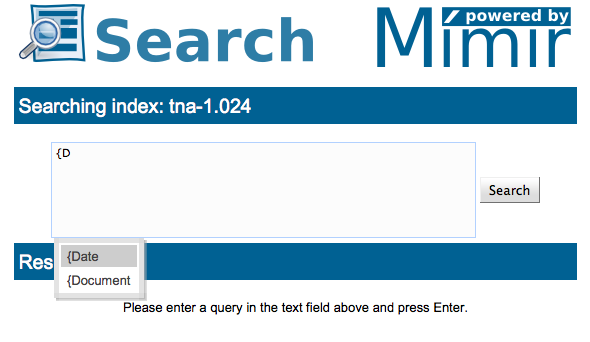
\includegraphics[scale=0.5]{img/gus-front-page}
\caption{Front page of the GUS user interface}
\label{fig:gus:front-page}
\end{center}
\end{figure}

Clicking the Search button starts a search on the server.  The query runs
asynchronously, collecting hits in the background until either 30 seconds have
passed or 1 million hits have been collected, at which point it stops.  To
restart the search, click the ``$>>$ keep searching'' link.

Hits are shown below the search box, as shown in figure~\ref{fig:gus:results},
with the hit text highlighted in bold and with five tokens of left and right
context.  The document title is a link, in this example to the original
document as the index was created with the ``Document URIs are external links''
option.  The ``cached'' link shows \Mimir's cached copy of the document, with
all the hits from that document highlighted in red.  For indexes where the
document URIs are not external links the document title would link directly to
the cached version and there would be no separate ``cached'' link.

\begin{figure}[tbp]
\begin{center}
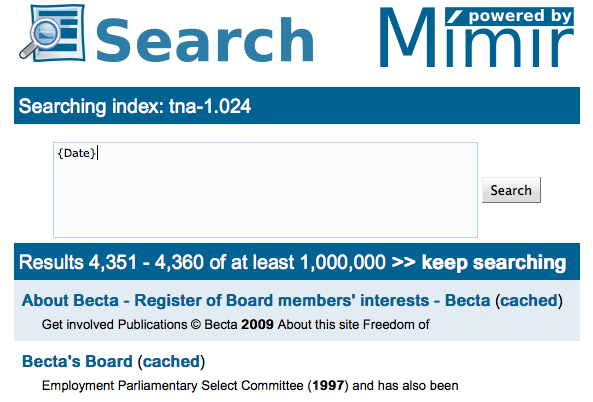
\includegraphics[scale=0.5]{img/gus-search-results}
\caption{GUS search results page}
\label{fig:gus:results}
\end{center}
\end{figure}

At the bottom of the page is a row of pagination links
(figure~\ref{fig:gus:pagination}).  Since, on a large index, there can be many
hundreds of thousands or even millions of hits to navigate, GUS provides links
where necessary to skip over large numbers of pages in one click.

\begin{figure}[tbp]
\begin{center}
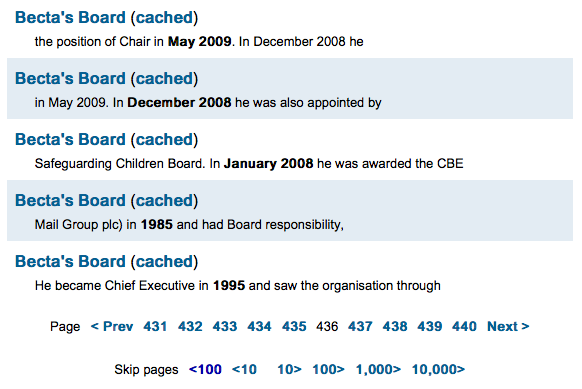
\includegraphics[scale=0.5]{img/gus-pagination-links}
\caption{GUS pagination links for a large search}
\label{fig:gus:pagination}
\end{center}
\end{figure}


%%%%%%%%%%%%%%%%%%%%%%%%%%%%%%%%%%%%%%%%%%%%%%%%%%%

\subsection{Embedding \Mimir\ in a Grails application}
\label{sec:search:grails}

Both the XML web service and the GUS interface ultimately use a Grails service
provided by the \Mimir\ plugin to search their indexes.  If you install the
\Mimir\ plugin into your own Grails application this service will be your
primary entry point to make use of \Mimir\ functionality, so this section
explains what you need to know to use it effectively.

The {\tt searchService} is a normal Grails service which can be autowired into
your own services, controllers, etc.  The service itself is very simple,
offering only the following methods:

\bde
\item[postQuery(index, queryString)] start running a query against the given
  index.  The index can be specified either as a string containing the indexId
  (the last component of the index URL, typically a UUID) or as an {\tt Index}
  domain object (the database object representing a local, remote or federated
  index).  Returns a {\em query ID} string.
\item[getQueryRunner(queryId)] retrieves the {\tt QueryRunner} for the given
  running query ID.  {\tt QueryRunner} is the interface through which you can
  interact with the running query.
\item[closeQueryRunner(queryId)] indicates that the given query runner is no
  longer required.  It is important to call this method when you have finished
  with a query runner, as each runner owns resources such as background threads
  which need to be properly cleaned up.
\ede

Once a query has been started, its {\tt QueryRunner} provides access to the
statistics, the hits themselves, and the text in the matched documents.  The
most important methods are summarised below, but for full details you should
look at the interface definition itself, in the {\tt gate.mimir.search} package
of {\tt mimir-core}.  Note that the search itself is performed in a background
thread so many of the methods of {\tt QueryRunner} will return different values
over time as the search progresses.

\bde
\item[isComplete()] Checks whether the search has completely finished and there
  are definitely no more hits to be found.
\item[isActive()] Checks whether the runner is currently actively searching.
  By default a query runner keeps searching until it has either exhausted all
  the possible hits, has found a million hits since it was last restarted, or
  has been running for 30 seconds without hitting this limit.  If isActive()
  and isComplete() both return false, it means that the search hit one of these
  limits and was suspended, it can be restarted by calling getMoreHits().
\item[getHitsCount()] Gets the number of hits obtained so far. This number may
  increase at any time if the query is currently active.
\item[getDocumentsCount()] Gets the number of distinct documents that have so
  far been found to contain hits.  This number may increase at any time if the
  query is currently active.
\item[getHits(start, max)] Gets the details of some hits found by the query.
  Conceptually, a {\tt QueryRunner} can be thought of as holding a flat list of
  hits numbered from zero upwards, containing all the hits from the first
  matched document, followed by all the hits from the second matched document,
  etc.  This method retrieves a sub-list from that list, starting at the
  (zero-based) index {\em start} and containing a maximum of {\em max} entries
  (it may contain fewer if not enough hits have yet been found).  The return
  value from this method is a list of {\tt Binding} objects, each representing
  one hit.
\item[getDocumentHitsCount(documentIndex)] Gets the number of hits in the $n$th
  document that matched this query (zero-based index).  To retrieve the hits
  for a particular document you would need to sum up all the
  getDocumentHitsCount values for the preceding documents and pass that sum as
  the {\em start} parameter to getHits.
\item[getDocumentID(documentIndex)] Gets the ID in the underlying index of the
  $n$th document that matched this query.  This ID is needed to get the
  document text and metadata.
\item[getDocumentTitle/URI(id)] Gets metadata about the document with the given
  ID.
\item[getDocumentText(id, start, length)] Gets the text of the document with
  the given ID, starting at the {\em start}th token and extending for
  {\em length} tokens.  The return value is a pair of parallel string arrays,
  one containing the text of the tokens and the other containing the text
  between each token and the following one.
\item[renderDocument(id, Appendable)] Render the document content, with hits
  highlighted, using the document renderer configured for the index.  The
  content is written to the specified Appendable (a StringBuilder, Writer,
  etc.).
\ede

The getHits method returns a list of {\tt Binding} objects, which provide
several methods, the most important ones being {\tt getDocumentId} (the
document that contains the hit), {\tt getTermPosition} (the offset of the first
token covered by the hit) and {\tt getLength} (the number of tokens it
covers).
